\section{Introduction}
\label{sec:intro}

\begin{figure}[t]
\centering
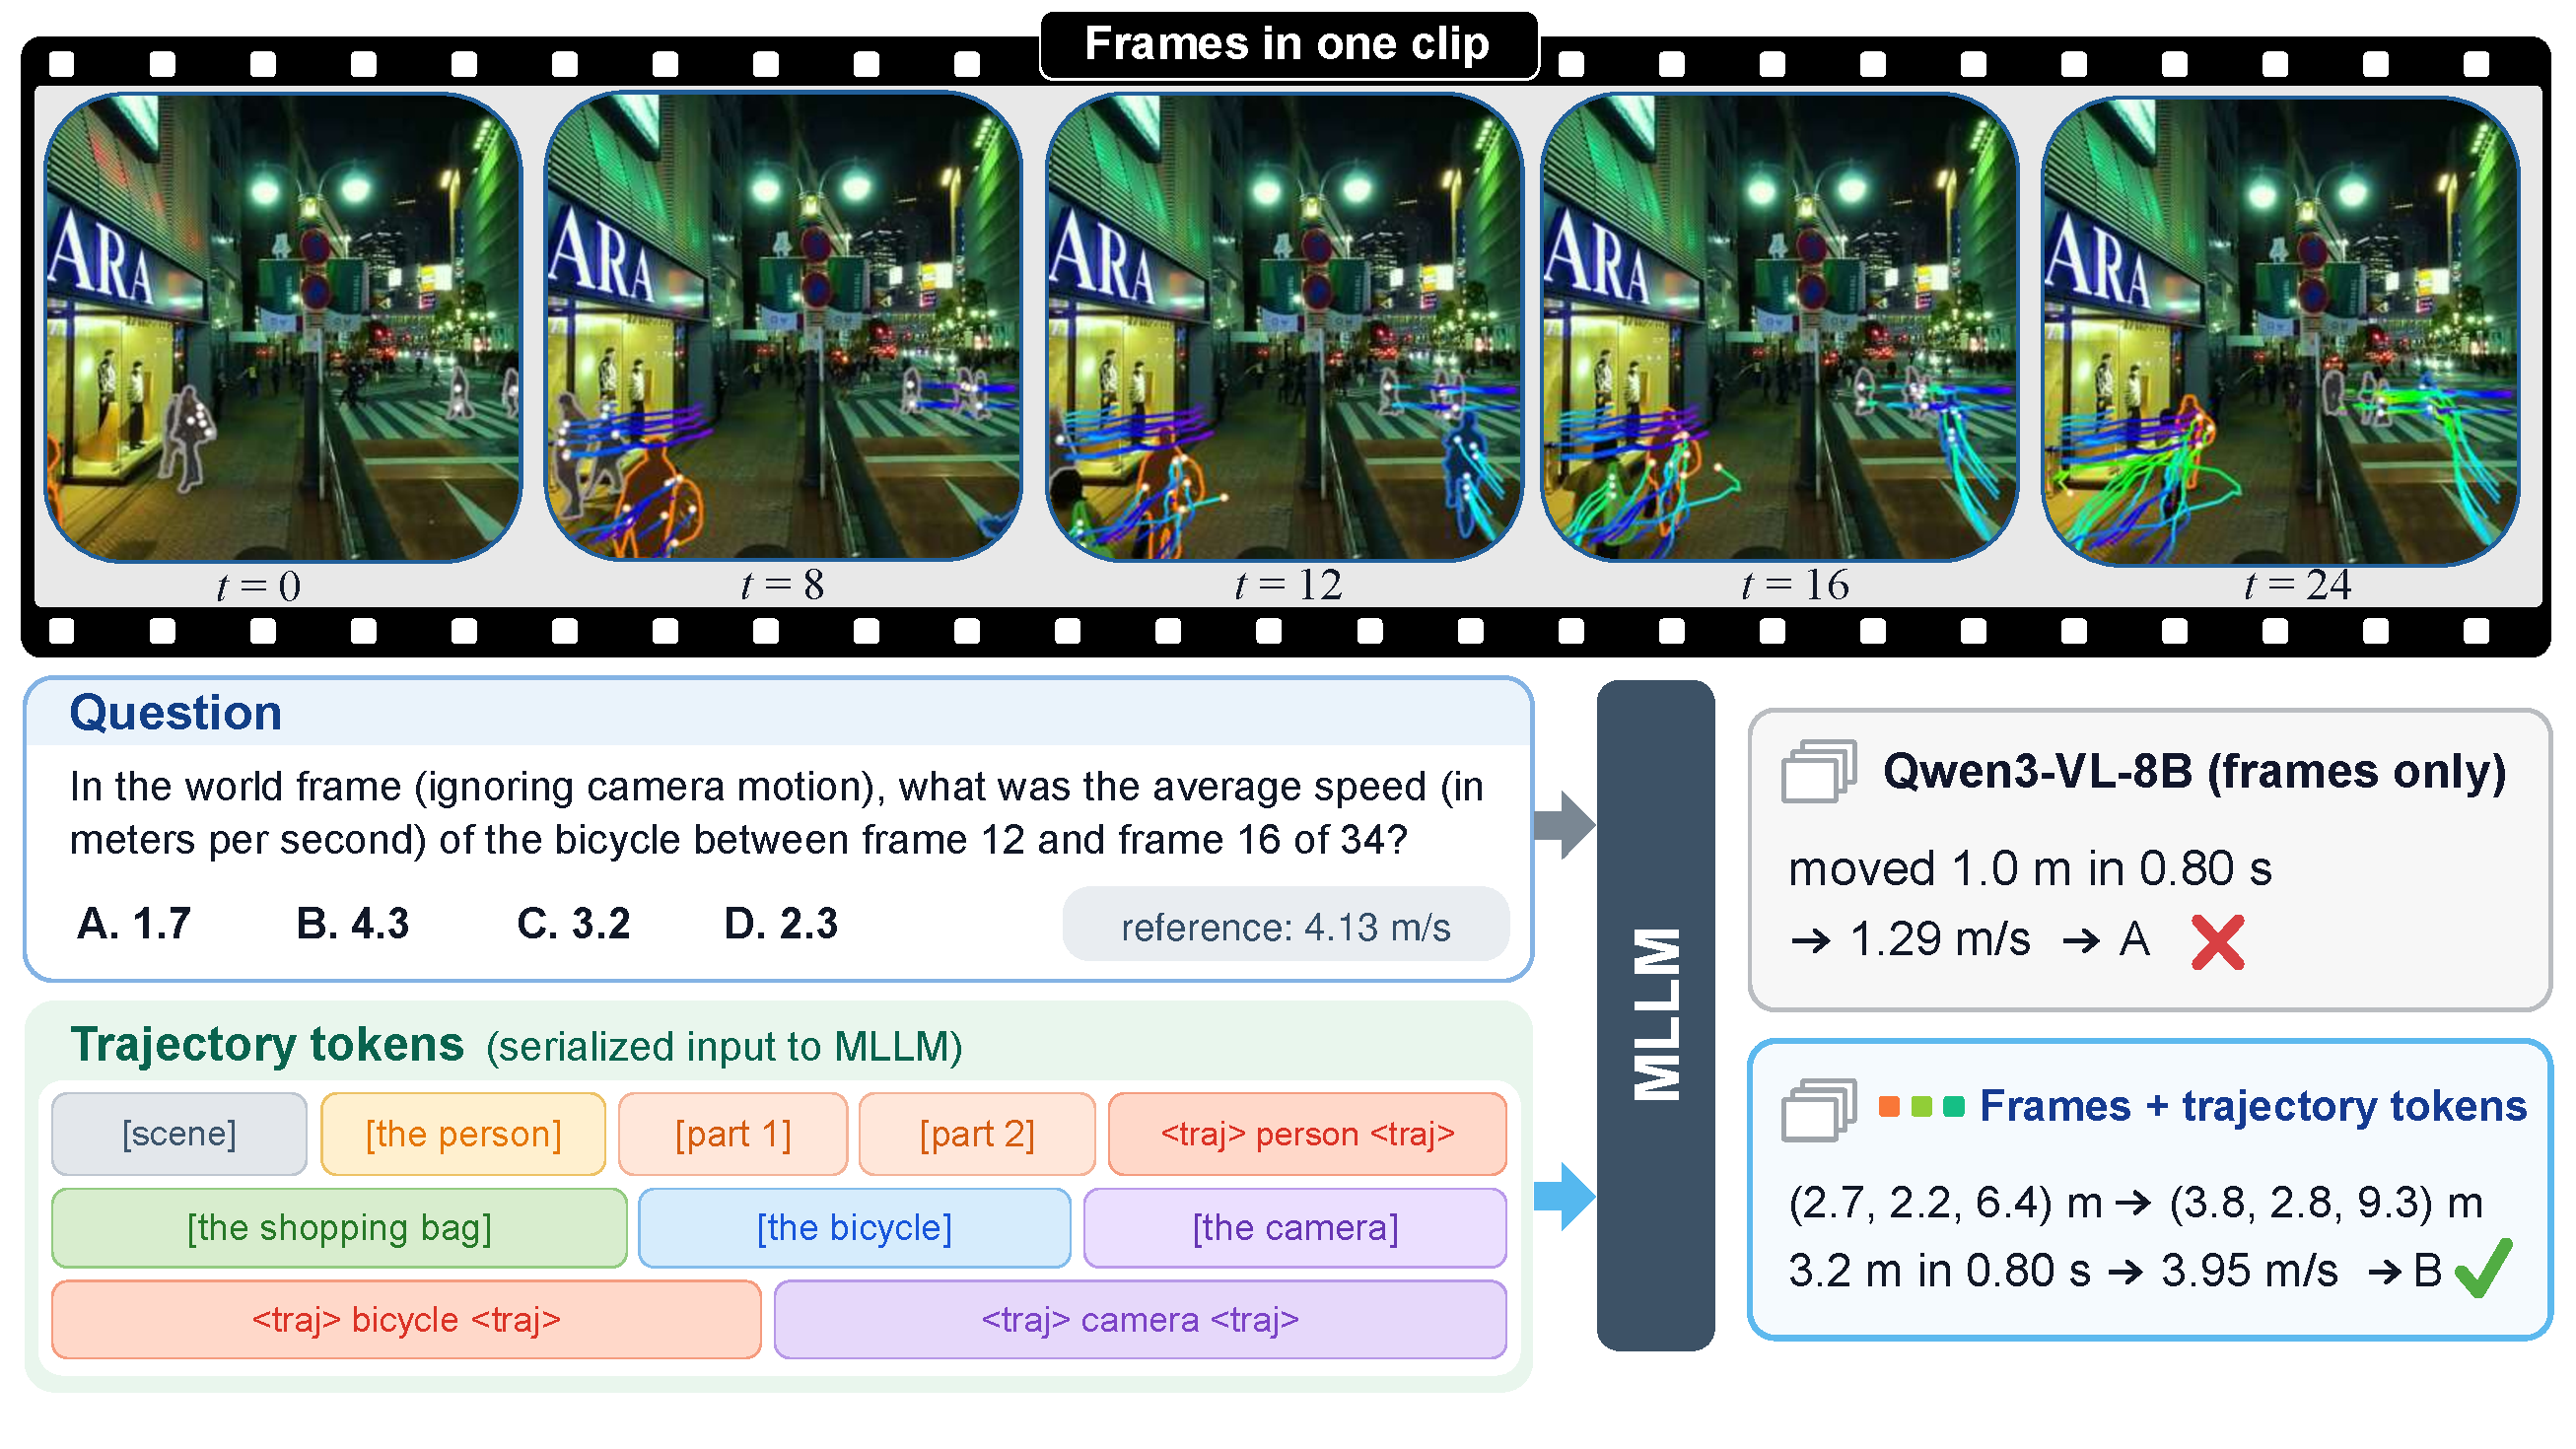
\includegraphics[width=\linewidth]{fig1_teaser_labels.pdf}
\caption{\textbf{Metric motion is hard to read from sampled frames.} Five frames and reconstructed 3D tracks accompany a question whose legacy \emph{average speed} wording is scored as endpoint displacement per elapsed second. Separately fine-tuned Qwen3-VL-8B arms predict 1.29~m/s from frames and 3.95~m/s from frames plus trajectory tokens; the reconstruction-derived reference is 4.13~m/s. The example illustrates the input setting, not an isolated causal effect of any one tokenization component.}
\label{fig:teaser}
\end{figure}

Understanding a dynamic scene requires reasoning about where objects are in three dimensions and how their positions change over physical time. A question such as \emph{How far did the person move between these frames?} needs metric scale, object identity, temporal correspondence, and separation of object motion from camera motion. These quantities matter for embodied agents, video search, and assistive scene understanding, but can be ambiguous in a short, sparsely sampled video. Contemporary multimodal language models (MLLMs) remain weak on spatial and spatiotemporal questions~\citep{yangThinkingSpaceHow2025,jiaOmniSpatialComprehensiveSpatial2026,liViSTRBenchCanMLLMs2026}. Figure~\ref{fig:teaser} shows the particular difficulty of recovering a numerical motion quantity from frames alone.

Most spatial MLLMs acquire geometric knowledge through images, depth, or video instruction tuning~\citep{chenSpatialVLMEndowingVisionLanguage2024,chengSpatialRGPTGroundedSpatial2024,caiSpatialBotPreciseSpatial2025}. Recent dynamic-scene models also incorporate reconstructed features or 4D questions~\citep{fanVLM3RVisionLanguageModels2026,yinMLLM4DVisualbasedSpatialTemporal2026}. Yet the model must still infer and retain the queried world-frame trajectory from a limited visual context. Conversely, 3D reconstruction can supply explicit point tracks, but naively listing hundreds of points across tens of frames overwhelms the language context and obscures which motion belongs to which object. This leaves an interface problem: how can an MLLM read compact, metric, object-grounded motion without having to recover it again from pixels?

We propose \emph{Sparse Trajectory Tokens}, an interface that turns externally reconstructed 4D motion into an ordered sequence of physical-time trajectory records. The central idea is to preserve the information needed for a motion query, including object and part identity, visible world-frame positions, time, and motion discontinuities, while spending tokens only where the track changes. This is a conditional setting: reconstruction is supplied at inference, and its accuracy bounds the answers the model can give.

The method has three connected modules (Fig.~\ref{fig:pipeline}). The \emph{Object-Centric Track Constructor} assigns reconstructed 3D tracks to segmented objects and chooses sparse, part-aware keypoints, separating object and camera motion. The \emph{Event-Aware Trajectory Tokenizer} normalizes the scene, preserves visibility gaps, splits salient changes, and adaptively fits piecewise curves whose on-curve samples become time-stamped tokens. The \emph{Trajectory-Language Adapter} embeds the records directly into an existing MLLM and trains it to describe motion and answer questions using the supplied values. Together they connect dense reconstruction to metric language output under a bounded token budget.

We evaluate this interface with TrajQA-B, a benchmark constructed from Stereo4D reconstructions~\citep{jinStereo4DLearningHow2025}. The questions ask for object or camera displacement and endpoint displacement per elapsed second, with answers checked against the serialized tokens. On 7,500 four-choice numeric questions, our trajectory-input model reaches 82.2\% accuracy; a separately trained frames-only arm reaches 48.3\%. Replacing the correct trajectories with another scene's records reduces accuracy to 29.6\%, and the generated numerical evidence becomes substantially less accurate. These results support effective reading of supplied trajectories. They do not establish the individual benefit of the spline, event, or part choices, for which controlled component ablations are still needed.

\paragraph{Contributions.} (1) We formulate an object-centred, part-aware interface from dense reconstructed 4D tracks to sparse world-frame motion records. (2) We introduce event-aware adaptive trajectory tokens and a direct token-to-language embedding adapter that retain metric scale and physical time within a compact sequence. (3) We construct TrajQA-B with token-side answer checks and report a separately trained frames-only reference, same-model input interventions, and metric evidence diagnostics that delimit what the model has learned.
